\chapter{Stratégie d'étude}\label{chap2}
\lhead{\emph{Stratégie d'étude}}


Les \textbf{S}ystèmes de \textbf{T}ransmission de l'\textbf{I}nformation \textbf{G}énétique (\textbf{STIG}) sont les mécanismes génétiques permettant la réplication, la ségrégation et la maintenance des réplicons au cours des générations. {\color{orange}\bf Le passage d'un génome monopartite à multipartite (ou inversement) doit logiquement passer par une adaptation des STIG du génome afin de permettre l'intégration de la réplication et de la ségrégation d'un chromosome additionnel (ou sa disparition) dans le cycle cellulaire et vis-à-vis de chromosomes préexistants}. Il apparaît alors pertinent de caractériser les réplicons et génomes bactériens selon les STIG qu'ils utilisent. Dans cette étude, nous recherchons plus spécifiquement à mettre en contraste les RECE par rapport aux chromosomes primaires (et chromosomes uniques) et aux “vrais” plasmides afin, premièrement, de discriminer efficacement les différentes catégories de réplicons et secondairement, d'identifier les systèmes-clés de l'émergence et de la stabilisation des génomes multipartites. 

\section{Les protéines des STIG: variables explicatives des réplicons}\label{parchap2introworkflow}
Les chapitres \ref{chap1a} et \ref{chap1b} ont présenté les STIG des réplicons bactériens, ainsi que la conception actuelle de l'architecture du génome bactérien. Il semble alors que les types de réplicon, et les espèces et écologies des organismes les hébergeant sont fonctionnellement liés à leurs STIG. \textbf{Selon notre postulat d'adaptation des STIG dans les génomes multipartites, des différences de distribution des gènes liés aux STIG entre génome mono- et multi-partites doivent être détectables par une analyse bioinformatique}. Nos données de départ étant l'ensemble des génomes bactériens séquencés disponibles dans les bases de données publiques, nous annotons dans un premier temps l'ensemble des gènes liés aux STIG dans ces génomes. En prenant ces gènes comme attributs des réplicons, nous analysons ensuite ce jeu de données pour identifier et caractériser d'éventuels biais de distribution entre les réplicons, afin, à partir de ces résultats, de distinguer les différents types de réplicons. Enfin, nous relions ces biais à des réalités biologiques et génomiques.
Deux types d'attributs sont utilisés pour caractériser les réplicons bactériens:
\begin{description}
\item[\textbullet]les groupes d'homologues des protéines liées au STIG, 
\item[\textbullet]les différentes fonctions de ces protéines.
\end{description}
Dans le premier cas, la mesure rapprochant deux protéines étant l'homologie de séquence, la proximité de deux réplicons traduira un lien évolutif potentiel. Dans le second cas, les réplicons seront identifiés selon leur fonctionnalité.

\section{Fondement de la génomique comparative}\label{introchap2}
Trois modalités d'analyse bioinformatique peuvent être distinguées:
\begin{itemize}
\item L'analyse de séquences biologiques (protéines, ARN, ADN), “analyse” sous-entendant la comparaison (recherche d'homologie) des séquences. 
\item La modélisation moléculaire qui consiste à inférer le comportement et/ou l'organisation de structures moléculaires.
\item La biologie des systèmes, cherchant à construire des modèles reliant différents niveaux d'information biologique (structural, moléculaire, écologique...).
\end{itemize}
\medskip
Un des paradigme fondamental est que l'\textbf{homologie} de séquence est liée à une origine évolutive commune des séquences comparées \citep{wray1998homology} et, à un degré moindre, à une \textbf{homologie fonctionnelle} \citep{chikina2011accurate}. Ces hypothèses permettent, par exemple, d'étudier les relations phylogéniques entre individus ou d'annoter une séquence biologique inconnue par rapport à des séquences biologiques déjà annotées.\\
L'homologie de deux séquences peut refléter différents mécanismes évolutifs:
\begin{description}
\item[$\bullet$ \textbf{Orthologie}] \citep{fitch1970distinguishing} Deux séquences chez deux organismes distincts sont orthologues si elles descendent d'une unique séquence ancestrale présente dans le dernier ancêtre commun aux deux espèces. L'homologie de deux gènes séparés par un événement de spéciation laisse supposer que les gènes ont conservé la fonction du gène ancestral et ont, \textit{a priori}, la même fonction.
\begin{figure}[H]
\Tree [.{\hspace{1cm}Gène $\alpha$ ancestral $\Longleftarrow\mathrm{\textbf{Spéciation}}$} {Gène $\alpha$ Espèce A} {Gène $\alpha$ Espèce B} ]
\subcaption{\textbf{Orthologie} entre les gènes $\alpha$ des espèces A et B.}\label{figrotho}
\end{figure}
\item[$\bullet$ \textbf{Paralogie}] \citep{fitch1970distinguishing} Deux g sont paralogues si elles résultent d'une \textbf{duplication génique}. On distingue de plus les \textbf{In-paralogues} si la duplication a eu lieu avant l'événement de spéciation, et les \textbf{Out-paralogues} si la duplication a eu lieu après la spéciation.
\begin{figure}[H]
\hspace{-1.5cm}
\begin{minipage}{0.5\textwidth}
\Tree [.{\hspace{1cm}Gène $\alpha$ ancestral $\Longleftarrow\mathrm{\textbf{Duplication}}$} {Gène $\alpha$ Espèce A} {Gène $\beta$ Espèce A} ]
\subcaption{\textbf{In-paralogie} entre les gènes $\alpha$ et $\beta$ de A.}\label{figinpara}
\end{minipage}
\begin{minipage}{0.5\textwidth}
\Tree [.{\hspace{1cm}Gène $\alpha$ ancestral $\Longleftarrow\mathrm{\textbf{Spéciation}}$} {Gène $\alpha$ Espèce A} [.{Gène $\alpha$ Espèce B $ \Longleftarrow\mathrm{\textbf{Duplication}}$} {Gène $\alpha$ Espèce B} {Gène $\beta$ Espèce B} ] ]\\
\subcaption{\textbf{Out-paralogie} entre le gène $\alpha$ de A et le gène $\beta$ de B.}\label{figoutpara}
\end{minipage}
\end{figure} 
\medskip
La duplication génique est souvent suivie d'une divergence fonctionnelle des gènes dupliqués. Un des gènes conserve la fonction du gène ancestral et l'autre diverge pour acquérir une nouvelle fonction \citep{fitch1970distinguishing,fitch2000homology}. 
\item[$\bullet$ \textbf{Xénologie}] Deux gènes sont xénologues si leur homologie traduit une histoire évolutive commune mais, pour l'une des espèces les hébergeant, n'est pas liée au gène présent dans l'ancêtre direct dont ces dernières sont issues. Dans les génomes bactériens, la présence de séquences xénologues témoigne fréquemment d'un transfert horizontal de gènes (THG) inter-réplicons et/ou inter-individus. L'évolution des génomes bactériens étant soumise à un flux important de THG (\citep{Bapteste2009,Doolittle2007}), la détection d'orthologues au sein des différents réplicons est souvent délicate et bruitée par les xénologues.
\end{description} 


\section{Concept du génome-cœur}\label{coregenome}
De nombreuses études mettent en avant la présence d'une collection de gènes homologues chez l'ensemble des membres d'une espèce (par exemple, pour \textit{Salmonella enterica} \citep{lan2009population} ou \textit{Helicobacter pylori}). Cela a conduit à la proposition de l'hypothèse du \textbf{génome-cœur} ou \textit{Core Genome Hypothesis} \citep{lan1996gene}. Cette théorie distingue la fraction du génome (le cœur) partagée par tous les membres de l'espèce, de la fraction auxiliaire qui est seulement présente dans une sous-population. Le génome-cœur définit ainsi les spécificités d'une espèce bactérienne. Les gènes du génome-cœur codent principalement les fonctions métaboliques essentielles et les processus cellulaires de transmission d'information \citep{Riley2009}. Ainsi, \textbf{une part importante des gènes des STIG sont inclus dans le génome-coeur des bactéries}. Les génes de la partie auxiliaire sont principalement les gènes codant des fonctions métaboliques supplémentaires, utiles dans le contexte de certaines écologies, et sont plus fréquemment associés à des plasmides ou des éléments mobiles \citep{Riley2009}.
\iffalse
single gene/motif detection: \citep{Brilli2010}.
TGH: \citep{Bosi2011}.
Association rules pour clustering et visualisation de données biologiques \citep{Karpinets2012}.
Phylogénomique: Besoin moderne de phylogénie \citep{chan2013next}.
Remote homologie detection \citep{Bernardes2011}.
Protéines organisées en domaines: Une combinaison de domaines similaires, témoigne-t-elle d'une même fonction, d'une origine commune ou est-elle due au hasard? \citep{song2008sequence}.
Théorie du core genome hypothesis? 
\fi

\section{Fouille de données en génomique}\label{analyseintro}

\subsection{Méthodes analytiques}
Avec l'explosion de la production de données génomiques, et en particulier l'avènement de nouvelles technologies de séquençage de l'ADN et des méthodes \textit{chip-seq}, les chercheurs sont confrontés à un afflux massif de données génomiques, transcriptomiques, protéomiques ou physiologiques. Cette avalanche de données est devenue un défit pour les bio-analystes et requiert le développement constant de méthodes analytiques permettant de traiter de façon pertinente (et de stocker) des quantités toujours plus importantes d'information génétique bruitée dans des temps raisonnables.\\
Les données à analyser sont souvent multivariées, \textit{i.e.}, décrites par une collection de paramètres (taux d'expression génique, présence/absence de gènes, écologie des organismes ...) généralement considérés comme des variables aléatoires. Parmi les méthodes d'analyse multivariée, on distingue les méthodes de statistiques classiques, impliquant des tests d'hypothèses, des méthodes dites de fouille de données (\textit{\textbf{data mining}}) généralement employées pour analyser des jeux de données massifs et multi-dimensionnels \citep{izenman2008modern}. Le terme \textit{data-mining} fait référence à un concept un peu “fourre-tout” englobant des approches de transformation et de préparation des données, de visualisation, d'extraction de connaissance et d'évaluation. Parmi ces méthodes d'analyses, nous pouvons distinguer les \textbf{méthodes descriptives}, qui ont pour objectif d'explorer les données (recherche d'observations aberrantes (\textbf{\textit{outliers}}), de structures ou de tendances, sélection de variables...), des \textbf{méthodes prédictives} où l'objectif est de construire un modèle à partir des données. Les méthodes de data-mining ont souvent recourt à des concepts statistiques, mais une part importante de ces méthodes englobe les approches dites d'apprentissage (\textbf{\textit{Machine Learning}}). À partir d'un jeu de données, les algorithmes prédictifs de machine learning cherchent à apprendre, à reconnaître des tendances complexes et sont capables de prendre des “décisions”' en fonction des données \citep{han2012data}. Une façon de conceptualiser les problèmes d'apprentissage est d'imaginer qu'est recherché à travers un espace de concepts descriptifs, un ensemble de règles décrivant au mieux un jeu de données \citep{witten2013data}. Ainsi, un algorithme de machine learning est défini par les différents concepts descriptifs utilisés pour représenter les données, l'ordre dans lequel est parcouru l'espace des concepts et la façon dont sont traités les problèmes de sur-apprentissage (ou \textbf{\textit{overfitting}}) des jeux de données d’entraînement (\textbf{\textit{training set}}) \citep{witten2013data}. Enfin, nous pouvons distinguer les méthodes d'\textbf{apprentissage supervisé} (classification ou régression), où un ensemble de variables d'entrée (\textbf{\textit{input}}) dont l'état de sortie (\textit{\textbf{output}}) est connu sert à entraîner un algorithme d'apprentissage afin de traiter des données dont l'état de sortie n'est pas connu, des méthodes d'\textbf{apprentissage non-supervisé} (clustering par exemple) où aucune information \textit{a priori} n'est disponible sur l'état de sortie des données. \\
\\
L'efficacité d'un algorithme peut être mesurée selon différents critères. Dans l'analyse de données biologiques, on peut souligner l'importance de: 
\begin{description}
\item[$\bullet$] \textbf{La complexité temporelle et spatiale}, c'est-à-dire la faisabilité temporelle et matérielle d'un algorithme. Cela ce traduit concrètement par le temps d'exécution d'un algorithme $t$, et la taille de la mémoire nécessaire $m$. Formellement les complexités temporelle et spatiale peuvent être représentées par des fonctions $O_{t}(Y)$ et $O_{m}(Y)$ indiquant que $t$ et $m$ vont être proportionnels à $Y$, où $Y$ s'exprime généralement en fonction du nombre de données à analyser $n$, et de la dimension des données $d$ ($Y=f(n,d)$). Les problèmes génomiques impliquant généralement des $n$ et $d$ importants, la complexité temporelle exponentielle ($O(e^{n.d}) $) d'un algorithme le rend souvent inutilisable en pratique. Il est alors important de déterminer si un problème informatique est divisible en plusieurs sous-problèmes autorisant sa parallélisation sur plusieurs processeurs. 
\item[$\bullet$] \textbf{La performance}. Les méthodes doivent fournir des résultats pertinents des points de vue statistique et biologique. Différents critères d'évaluation peuvent être utilisés, tels que, par exemple, l'erreur de prédiction ou de généralisation \citep{izenman2008modern} ou la stabilité ou l'insensibilité à l'ordre des entrées \citep{Andreopoulos2009}. Une propriété importante des méthodes prédictives est leur capacité à généraliser le modèle construit à partir du training set à des jeux de données inconnus. La \textbf{robustesse} des algorithmes est la capacité à générer des résultats pertinents quand les entrées sont des données “bruitées” dans les cas, par exemple, des valeurs manquantes ou singulières \citep[Chap. 8]{han2012data};\citep{Andreopoulos2009}. 

\item[$\bullet$] \textbf{Le nombre de paramètres à définir}. Les paramètres que doit définir l'utilisateur d'un algorithme peuvent affecter les résultats d'une manière significative \citep{Andreopoulos2009}. Afin de minimiser les erreurs dues aux choix de l'utilisateur, il peut être préférable qu'un algorithme utilise un nombre limité de paramètres à définir.

\item[$\bullet$] \textbf{ L'inclusion de variables multicatégories}. Il est souvent utile en génomique comparative de pouvoir prendre en compte des variables de différents types: par exemple, des groupes de gènes d'une part, et des critères écologiques ou morphologiques d'autre part. 
\end{description}

\subsection{Notations}
On note $E=\{e_{1},...,e_{n}\}$, l'ensemble $E$ des $n$ éléments $e_{i}$ avec $1<i<n$ de taille $|E|=n$. On peut alors écrire: $E=\{e_{1},...,e_{|E|}\}$ lorsque $n$ n'est pas connu.\\
\\
On note $v=(x_{1},...,x_{n})$, le vecteur $v$ de taille $|v|=n$ avec $x_{i}$, les différentes valeurs de $v$ avec $1<i<n$ et $x_{i}$ appartenant à $\mathbb{R}$ ou $\mathbb{N}$. $v$ appartient alors à $\mathbb{R}^{n}$ ou $\mathbb{N}^{n}$.\\
\\
On note de plus $v[i]=x_{i}$. Pour un ensemble $V=\{v_{1},...,v_{|V|}\}$ de vecteurs $v_{i}$ de même taille $n$, on note $M^{V}$ sa matrice de dimension $(|V|,n)$ telle que $M^{V}_{i,j}=v_{i}[j]$, avec $1<i<|V|$ et $1<j<n$. \\
\\
Pour un ensemble de données, le terme \textbf{observation} désigne une donnée tirée de cet ensemble. Les observations étant souvent représentées par des vecteurs, le terme \textbf{attribut} désigne alors les variables descriptives de ces vecteurs. Pour un ensemble d'observations $E=\{e_{1},...,e_{|E|}\}$ définies par $n$ attributs $X=\{X_{1},...,X_{n}\}$, l'ensemble $V^{E}=\{v^{e_{1}},...,v^{e_{|E|}}\}$ désigne l'ensemble des vecteurs d'observations où $v^{e_{i}}[j]$ est égal à la valeur du $j$-ième attribut pour l'observation $e_{i}$. 


\subsection{Distances}
Pour comparer deux observations, plusieurs distances \citep{gan2007data} peuvent être calculées selon leurs attributs et les propriétés souhaitées:\\
\\
Si les observations sont deux ensembles $E_{1}$ et $E_{2}$, la distance de Jaccard peut être utilisée: 
\begin{equation}
d_{Jaccard}(E_{1},E_{2})=1-\frac{|E_{1}\cap E_{2}|}{|E_{1}\cup E_{2}|}
\end{equation}
\\
Pour deux observations $v_{1}$ et $v_{2}$ ayant des attributs numériques, et de taille similaire $n$, la distance la plus couramment utilisée est la distance Euclidienne:
\begin{equation}
d_{Euclid}(v_{1},v_{2})=\sqrt{\sum_{1\leq i\leq n}{(v_{1}[i]-v_{2}[i])}^{2}}
\end{equation}
\\
Cette distance n'est pas forcément pertinente pour comparer des observations de très grande dimension dont une partie n'a aucun attribut en commun. On introduit donc une distance Euclidienne modifiée:
\begin{equation}\label{eqeuclidmodif}
d_{Euclid*}(v_{1},v_{2},Seuil)=
\begin{dcases} 
d_{Euclid}(v_{1},v_{2}) & \textrm{ si }\prod_{1\leq i\leq n}(v_{1}[i].v_{2}[i])\neq 0\\
Seuil & \textrm{ sinon}
\end{dcases}
\end{equation}
\\
Une distance est considérée comme \textit{métrique} si elle respecte les propriétés suivantes:
\begin{description}
\item[ Symétrie:] $d(a,b)=d(b,a)$
\item[ Séparation:] $d(a,b)=0 \;\Leftrightarrow \;a=b$
\item[ Inégalité triangulaire:] $d(a,c) \leqslant d(a,b)+d(b,c)$
\end{description}
Les distances de Jaccard et Euclidienne sont métriques. Cette propriété n'est pas toujours pertinente pour des données de dimension élevée et clairsemées (avec beaucoup d'attributs nuls). La distance \textit{cosine} (non métrique car ne respectant pas la dernière propriété) est alors souvent utilisée afin de se focaliser sur les attributs non nuls \citep{han2012data}:
\begin{equation}
d_{cosine}=1-\frac{\sum_{1\leq i\leq n}v_{1}[i].v_{2}[i]}{\sqrt{\sum_{1\leq i\leq n}{v_{1}[i]}^{2}}.\sqrt{\sum_{1\leq i\leq n}{v_{2}[i]}^{2}}}\label{eqcosine}
\end{equation}


\subsection{Méthodes de clustering}\label{parclusterintro}
Soit un ensemble $E$. On appelle procédure de clustering une procédure $f_{clust}$ qui structure un ensemble d'observations en $k$ sous-ensembles ou \textbf{clusters} constitués des observations présentant des similitudes, sans \textit{a priori} sur la structure:
\begin{equation}
f_{clust}(E) =\{E_{1},...,E_{k}\} \textrm{ où:} \bigcup_{E_{i} \in f_{clust}(E)}E_{i}  = E
\end{equation}
De nombreux algorithmes de clustering existent \citep{gan2007data}. Les inputs de ces algorithmes peuvent être, entre autres, la distance utilisée. Cependant, un des paramètres clé souvent requis est le nombre $k$ de clusters à former.


\subsection{Méthodes de classification}\label{parclassifintro}
Une procédure de classification prend en input un training set $E_{training}$, constitué de différents sous-ensembles (ou classes) d'observations: $E_{training}=\{E_{1},...,E_{k}\}$, et construit à partir de cet ensemble un modèle permettant d'attribuer à une observation $o$, une des classes de $E_{training}$. Soit $E_{test}$ un ensemble d'observations, et $E_{training}$ un training set tel que $\forall E \in E_{training},\; E \subset E_{test}$. Une procédure de classification $f_{classif}^{E_{training}}$ utilisant $E_{training}$ peut alors être alors définie par:
\begin{equation}
f_{classif}^{E_{training}}(o) = i,\:\: o \in E_{test} \textrm{ et } 1\leq i \leq k
\end{equation} 
L'objectif sous-jacent est, pour tout $E_{i} \in E_{training}$ et tout $o_{i} \in E_{i}$, de bâtir un classifieur tel que $f_{classif}^{E_{training}}(o_{i})=i$, se comportant de manière stable et robuste, et évitant l'\textit{overfitting} de $E_{training}$. Différents algorithmes de classification sont présentés plus loin. Une description plus complète de ces méthodes est disponible dans \citep{han2012data,witten2013data}.
\subsection{Projection}\label{parproj}
Une procédure de projection consiste à projeter des observations représentées dans un espace de dimension $p$, dans un nouvel espace de dimension $q$ avec $q<p$.\\
Soit $f_{P}^{q}$ la procédure de projection $P$ de données provenant d'un espace $Q^{p}$ de dimension $p$ dans un espace $Q'^{q}$ de dimension $q$. Pour une observation $v=(x_{1},...,x_{p})$ décrite par $p$ attributs avec $v \in Q^{p}$ et $x_{i} \in Q$, on définit $f_{P}^{q}$ par :
\begin{equation}
f_{P}^{q}(v)=(y_{1},...,y_{q}) \textrm{ où } y_{i} \in Q'
\end{equation}
Ici $Q \in \{\mathbb{R},\mathbb{N}\}$ et Q' est l'ensemble des réels $\mathbb{R}$. Pour un ensemble d'observations $V=\{v_{1},..,v_{|V|}\}$, on définit $M^{V}_{P}$ par:
\begin{equation}
M^{V}_{P}=f_{P}^{q}(V)=\{f_{P}^{q}(v_{1}),...,f_{P}^{q}(v_{|V|}) \} \textrm{ où } v_{i} \in V
\end{equation} 
Une procédure de projection peut être utilisée dans le but de représenter des données dans un espace interprétable et visuel. Dans ce cas, $q$ est classiquement fixé à 2 ou 3. Ici, les données sont visualisées dans un espace à deux dimensions en fixant $q$ à 2.


\subsection{Évaluation}\label{analyseeval}
L'efficacité d'une analyse bioinformatique peut être appréhendée de deux manières: i) d'un point de vue informatique et statistique, où l'on mesure la performance des résultats selon différents critères, et ii) d'un point de vue biologique, où l'on cherche à voir si les résultats sont significatifs biologiquement et non un artefact découlant, par exemple, d'un biais initial dans les données (sur-représentation d'une classe, données manquantes...).

\subsubsection{Performance des classifieurs}\label{parperf}\label{parclassifrobust}
L'évaluation de la performance des méthodes de classification se fait \textit{via} l'évaluation de différents indices à partir des résultats apportés par les classifieurs et selon des procédures spécifiques. En considérant les résultats d'un classifieur sur un training set, soient $TP$ et $FP$, les résultats vrais ($T$ pour "true") annotés positivement ($P$) et négativement ($N$), et $FP$ et $FN$, les résultats faux ($F$ pour "false") annotés positivement ($P$) et négativement ($N$), respectivement. Nous pouvons définir les mesures suivantes \citep{han2012data,hamel2011knowledge}:
\begin{equation}\label{eqsensitive}
\begin{split}
\textrm{sensibilité} & =\frac{TP}{TP+FN}\\
\\[-0.2cm]
\textrm{précision} & =\frac{TP}{TP+FP}\\
\\[-0.2cm]
\textrm{spécificité} & =\frac{TN}{TN+TP}\\
\\[-0.2cm]
erreur & =\frac{TP+TN}{FP+FN+TP+TN}\\
\\[-0.2cm]
F-{measure} & =\frac{2.precision.sensibilite}{precision+sensibilite}\\
\end{split}
\end{equation}
\\
Ces estimateurs ne témoignent pas de la capacité d'un classifieur à se généraliser à des données indépendantes de celles du training set utilisé pour sa construction, de bons résultats pouvant simplement témoigner d'un \textit{overfitting} du classifieur sur le learning set initial. La capacité à se généraliser d'un classifieur peut être estimée en partitionnant le learning set initial en différents $E_{test}$ et $E_{learning}$ et évaluant les performances du classifieur sur les $E_{test}$ formés. Les procédures de validation croisée \textit{\textbf{cross-validation}} sont des procédures suivant ce principe \citep{witten2013data,han2012data,hamel2011knowledge}. La méthode \textbf{Leave-One-Out} (\textbf{LOO}) consiste à effectuer $n$ classifications sur les $n$ données du training set où, à chaque fois, une donnée (ou point) différente est classée en utilisant les $n-1$ autres données comme nouveau training set. La méthode \textbf{K-fold} consiste à séparer le training set en $K$ partitions et à effectuer $K$ classifications en testant à chaque fois une partition par rapport aux $K-1$ autres. La performance peut alors être mesurée avec, par exemple, les indices décrits. Une forte sensibilité, spécificité et précision (et donc un F-score important), et une faible erreur témoigneront d'un classifieur performant.
\\
Afin d'estimer si deux classifieurs présentent des performances différentes, des procédures de ré-échantillonnage de type \textbf{bootstrap} (ré-échantillonnage avec remise du training set initial) peuvent être effectuées où, pour chaque procédure, une nouvelle cross-validation est réalisée et sert à construire une distribution des scores obtenus pour les différents indices (notamment l'erreur de classification). Les distributions obtenues serviront alors à comparer les modèles (par des modèles statistiques de type test d'hypothèses) afin de choisir le plus performant \citep{hamel2011knowledge,han2012data}. Le bootstrap peut aussi servir de procédure de type cross-validation \citep{han2012data}.
\\
Les modèles de cross-validation LOO, K-fold et de bootstrap sont les principales représentantes d'une famille plus large de méthodes plus ou moins bien adaptées aux différents problèmes de classification \citep{arlot2010survey}. Ces modèles sont cependant eux-mêmes soumis à une sélection de paramètres ($K$ par exemple pour K-fold), pouvant être source d'erreur. Une façon d'améliorer les performances d'un classifieur est d'utiliser les méthodes dites d'\textit{\textbf{Ensemble}} dont le principe se réfère à des procédures de ré-échantillonnage des données et/ou des variables, et en combinant les scores obtenus pour chaque échantillon \citep{han2012data}. Les procédures de \textit{\textbf{Bagging}}, \textit{\textbf{Boosting}} ou encore les \textbf{forêts d'arbres aléatoires} (\textit{random forest}) font partie des méthodes d'\textit{Ensemble} les plus connues. Le choix d'un modèle particulier étant lui-même source de biais, la sélection d'une procédure d'évaluation de la performance et de la robustesse d'un classifieur est alors un compromis entre faisabilité, complexité et précision \citep{arlot2010survey}. Enfin, selon les classifieurs utilisés, différentes techniques permettent d'évaluer la probabilité d'appartenance d'une donnée à une classe donnée \citep{ruping2004simple,wu2004probability}. 

\subsubsection{Performance des algorithmes de clustering}\label{parclustperf}
L'estimation de la performance d'une solution de clustering est généralement soumise à deux types de critères.
\paragraph{Les critères de validation externe} \citep{han2012data,gan2007data} où les résultats du clustering $Cl$ sont comparés à ceux d'un autre clustering de référence $R$ construit, par exemple, par des experts ou dérivé d'un autre algorithme de clustering et/ou avec d'autres variables. En général, une mesure de validation externe prendra en compte deux critères:

\begin{description}
\item[$\bullet$ l'\textit{\textbf{homogénéité}}] des clusters mesurant la capacité des clusters $C_{i} \in Cl$ à contenir des données homogènes envers un cluster $R_{j} \in R$ du clustering de référence.
\item[$\bullet$ l'\textit{\textbf{exhaustivité}}] des clusters mesurant inversement l'homogénéité des $R_{j} \in R$ envers les $C_{i} \in Cl$.
\end{description}

Deux critères additionnels peuvent également être pris en compte: la \textbf{catégorie bruit} représentant un cluster $C_{bruit} \in Cl$ et incluant les éléments ne correspondant à aucun $C_{i}$, et la \textbf{préservation des petits clusters}. Différents indices ont été développés afin de comparer deux solutions de clustering \citep{gan2007data,rendon2011internal}. Pour $a$, le nombre de paires ayant des points dans le même cluster dans $Cl$ et $R$, pour $b$, le nombre de paires où les points sont dans le même cluster dans $Cl$ mais pas dans $R$ et $c$, inversement, et pour $d$, le nombre de paires où les points sont dans différents clusters dans $Cl$ et $R$, on obtient au total $M$ paires où $M=a+b+c+d=\frac{n(n-1)}{2}$. Des indices simples de validation externe peuvent alors être définis \citep{gan2007data}:\\
\begin{equation}
\begin{split}
\text{Statistique de Rand:\;} & R=\frac{a+d}{M}\\
\\[-0.2cm]
\text{Coefficient de Jaccard:\;}& J=\frac{a}{a+b+c}\\
\\[-0.2cm]
\text{Indice de Flokes et Mallows:\;}& FM=\sqrt{\frac{a}{a+b}.\frac{a}{a+c}}\\
\end{split}
\end{equation}
\paragraph{Les critères de validation interne} \citep{rendon2011internal,gan2007data} mesurant la qualité d'un clustering uniquement à partir des caractéristiques intrinsèques de la partition des données obtenues. En général, ces indices combinent deux concepts \citep{rendon2011internal}: i) la \textit{compacité} qui mesure la proximité des éléments au sein d'un même cluster (typiquement la variance intra-cluster), et ii) la \textit{séparabilité} qui mesure la distance séparant deux clusters distincts. De nombreux indices internes ont été développés \citep{rendon2011internal,gan2007data} et comme illustration, nous pouvons présenter le \underline{coefficient silhouette} \citep{rousseeuw1987silhouettes} qui est un estimateur interne classique. Pour un clustering $Cl$ de $n$ données et pour un point $i$ dans un cluster $C_{j}$, une mesure de qualité $s(i)$ peut être calculée: 
\begin{equation}\label{eqsilhouette}
\begin{split}
s(i)&=\frac{(b(i)-a(i))}{Max\{a(i),b(i)\}}\\
%\begin{dcases}
\text{avec $a(i)$ et $b(i)$:}\\
a(i)&=\frac{\sum_{j \in C_{i},j\neq i}d(i,j)}{|C_{i}-1|}\\
b(i)&=min\{\frac{\sum_{j \in C_{k}}d(j,i)}{|C_{j}|}\;| C_{k} \in Cl \textrm{ et } C_{k} \neq C_{i}\}
%\end{dcases}
\end{split}
\end{equation}
où $a(i)$ représente la distance moyenne entre $i$ et tous les autres points de $C_{j}$ et $b(i)$ est le minimum de la distance entre $i$ et les distances moyennes des points des clusters $C_{k,k\neq i}$. Cette mesure permet d'estimer la pertinence de la classification de chaque point dans un cluster. Elle varie entre -1 et 1. Des valeurs proches de 1 indiquent une pertinence élevée, et inversement, des valeurs négatives indiquent que $i$ est plus proche du centroïde d'un autre cluster. La moyenne des $s(i)$ d'un cluster donne un estimateur de la pertinence du cluster et la moyenne de tous les $s(i)$ procure un estimateur du clustering.
Un des problèmes majeurs généralement rencontré dans l'estimation de ces indices est qu'ils ont des complexités temporelles et/ou spatiales difficilement applicables sur des jeux de données très larges. Afin d'estimer la pertinence d'une analyse de clustering, certaines procédures ont été développées pour déterminer si la distribution des données est proche d'une distribution aléatoire, ce qui témoignerait d'une absence de structuration \citep{gan2007data,han2012data}. Plusieurs méthodologies et critères de validation relatifs permettent de comparer l'efficacité de différents algorithmes ou paramètres à produire des clusters pertinents d'un point de vue statistique \citep{gan2007data,kovacs2005cluster}. Notamment, certains auteurs ont proposé d'étudier la stabilité d'un clustering, l'idée générale étant de réaliser différents clustering d'un jeu de données en utilisant des méthodes de ré-échantillonnage (type bootstrap) et de mesurer la stabilité des clusters obtenus à travers les différents clustering \citep{hennig2007cluster,Hennig2008,Fang2012}.

\paragraph{Choix des paramètres}
Une difficulté généralement rencontrée dans une analyse de clustering est de déterminer le nombre de clusters à considérer, qui n'est pas connu \textit{a priori}. Le choix du nombre optimal de clusters $k_{opt}$ se fait alors en comparant l'efficacité des indices de robustesse pour différents $k$ \citep{Tibshirani2005,rakhlin2007stability,Fang2012}. Il est cependant important de ne pas perdre de vue qu'un clustering robuste et performant d'un point de vue statistique peut être complètement dépourvu de sens biologique, celui-ci pouvant correspondre à des artefacts dûs au jeu de données et/ou à l'algorithme utilisé \citep{hennig2007cluster}.

\subsection{Fléau de la dimensionalité}\label{parfleau}
Une des spécificités des données génomiques est qu'elles sont généralement de grande dimension (typiquement nos jeux de données ont des dimensions de l'ordre de 100 à 5000). Or, dans un espace de très grande dimension, le nombre de données disponibles est relativement peu élevé par rapport à la taille de l'espace de recherche. Les données ont alors tendance à se retrouver isolées \citep{izenman2008modern}. Un des problèmes pratiques qui en découle est que lorsque l'on veut, par exemple, mesurer la distance $d$ séparant quatre points $p1$, $p2$, $p3$ et $p4$ dans un espace de très grande dimension, en supposant qu'il existe certaines caractéristiques communes entre $p1$ et $p2$ dans certaines dimensions, mais aucune entre $p1$ ou $p2$ d'une part et $p3$ ou $p4$ d'autre part, ni entre $p3$ et $p4$, la distance $d(p1,p2)$ ne reflétera pas forcément la proximité de $p1$ avec $p2$ en comparaison de $d(p3,p4)$ à cause du bruit potentiellement engendré par les autres dimensions. Dans le cadre du data-mining, cela se traduit par la nécessité d'avoir d'énormes quantités de données, afin d'explorer au maximum l'espace de représentation des données pour avoir un modèle robuste \citep{izenman2008modern}. Une façon de contourner ce phénomène est de choisir des modèles et/ou des distances adaptés, comme par exemple un espace de dimension réduit ou des algorithmes spécifiques \citep{gan2007data}.
\\
\textit{\textbf{Cas d'exemple:}\\ 
Soient quatre vecteurs $p1=(5,3,0,0,0,0)$, $p2=(3,5,0,0,0,0)$, $p3=(0,0,0,0,0,1)$, et $p4=(0,0,0,0,1,0)$. Les distances euclidiennes calculées sont:
\begin{center}
\begin{tabular}{lllll}
& \textbf{p1} & \textbf{p2} & \textbf{p3} & \textbf{p4}\\
\textbf{p1} & 0\\
\textbf{p2} & 2.83 & 0\\
\textbf{p3} & 5.92 & 5.92 & 0\\
\textbf{p4} & 5.92 & 5.92 & 1.41 & 0\\
\end{tabular}
\end{center}
On constate que $d(p1,2)>d(p3,p4)$ même si $p1$ et $p2$ possèdent des caractéristiques communes (dans les deux premières dimensions) contrairement à $p3$ et $p4$ qui n'ont rien en commun.}
\subsection{Graphes}\label{chap2graph}
Les graphes sont des outils mathématiques de représentation de données et/ou de concepts qui peuvent être employés sur de nombreux jeux de données génomiques. L'ensemble des similitudes protéine-protéine d'un jeu de séquences est facilement représenté par un graphe (\textit{noeuds} = protéines et \textit{arêtes} = similitudes, qui peuvent être pondérées) qui peut ensuite être utilisé pour la visualisation des données ou faire des analyses de clustering \citep{Brohee2006,li2010computational}. Les graphes peuvent de plus être utilisés pour représenter des relations entre individus ou génomes comme par exemple, pour représenter un taux de THG ou des relations taxonomiques \citep{Lima-Mendez2008}. Formellement, un graphe peut être décrit de la façon suivante \citep{naim2011reseaux}: \\
Soit $N=\{e_{1},\dots,e_{|E|}\}$, un ensemble non vide d'éléments finis. Un graphe $G$ sur $N$ peut être défini par la donnée du couple:
\begin{equation}
G=(N,A) \textrm{ où } A \subset \{(e_{i},e_{j}) |\; e_{i},e_{j} \in N \textrm{ et } e_{i} \neq e_{j}\}
\end{equation}
$N$ est alors nommé l'ensemble des \textbf{nœuds} de $G$. $(e_{i},e_{j}) \in A$ est appelé une \textbf{arête} si et seulement si $(e_{j},e_{i}) \in A$ et un \textbf{arc}, sinon. Un graphe pondéré, $G_{w}$, est défini par $G_{w}=(N,A,W)$ où $W$ est une matrice carrée de taille $|N|*|N|$, appelée \textbf{matrice d'adjacence}, et $W_{ij}$, la valeur associée au couple $(e_{i},e_{j}) \in A$ ($W_{ij}=0$ si $(e_{i},e_{j}) \notin A$). La \textbf{distance géodésique} entre deux nœuds est le plus court chemin entre ces nœuds \textit{via} les arêtes (et leurs longueurs) du graphe \citep{han2012data}. Un graphe peut de plus être décomposé en partitions de noeuds où, à l'intérieur d'une partition, les noeuds sont indépendants et non connectés par des arêtes ou des arcs. De tels graphes sont appelés des \textbf{graphes multipartites}. En particulier, pour un ensemble d'observations $E=\{e_{1},...,e_{|E|}\}$ définies par un ensemble d'attributs $X=\{X_{1},...,X_{|X|}\}$ et représentées par un ensemble de vecteurs $V^{E}=\{v_{e_{1}},...,v_{e_{|E|}}\}$, on peut définir un graphe bipartite pondéré $G_{w}=(N,A,W)$ de la manière suivante:
\begin{equation}\label{eqbipartite}
\begin{dcases}
N=E \cup X\\
A= \{(e_{i},X_{j}) |\; v^{e_{i}}[j] \neq 0 \} \\
W_{ij} = v^{e_{i}}[j]
\end{dcases}
\end{equation}
où $e_{i} \in E$ et $X_{j} \in X$.\\
\\
Les graphes possèdent des méthodes d'analyse propres. Les méthodes dites de \textit{détection de communautés} font référence aux méthodes de partitionnement de graphes et sont assimilables aux méthodes de clustering \citep{Coscia2011}. Une communauté de nœuds peut être vue comme un ensemble de nœuds partageant des caractéristiques communes au sein d'un réseau. Différents critères peuvent alors servir à évaluer le taux de similitude entre différents nœuds \citep{Coscia2011}.


\subsection{Sources de biais}
Tout problème de data-mining peut être vu comme le calcul d'un estimateur $\hat{\theta}$ d'une certaine statistique $\theta$. Les biais de l'estimateur peuvent alors être définis par: 
\begin{equation}
Biais(\hat{\theta})\equiv E[\hat{\theta}]-\theta
\end{equation}
Dans une analyse de machine learning, les sources de biais possibles sont les suivantes \citep{witten2013data}: 
\begin{description}
\item[\textbullet]\small les différents concepts descriptifs utilisés pour représenter les données,
\item[\textbullet]\small l'ordre dans lequel est parcouru l'espace des concepts,
\item[\textbullet]\small la façon dont sont traités les problèmes de sur-apprentissage.
\end{description}
La première source de biais est concrètement exprimée par le choix et l'exhaustivité des données génomiques. Dans le cas de notre étude, ces données sont représentées par les réplicons choisis, les protéines sélectionnées en rapport avec les STIG et, dans un second temps, les clusters de protéines obtenus. La deuxième source de biais vient du choix des méthodes utilisées pour les analyses (clustering, classification, régression). Enfin, la troisième source de biais est la sélection des paramètres des méthodes pour éviter qu'ils ne soient pas trop spécifiques aux données. {\color{orange}\bf Ainsi, l'interprétation des résultats analytiques devra se faire en toute connaissance des différentes sources potentielles de biais.} 


\iffalse Enfin il existe une relation entre stabilité, variance et biais. L'instabilité d'un estimateur se traduisant généralement par une variance élevée (car perturbé) et un faible biais qui est la cause d'un overfitting des données. Inversement un large biais est généralement la conséquence d'un \textit{underfitting} des données \citep[p.505]{izenman2008modern}.\fi
% Bruit dans les données biologiques en général: \citep{Sloutsky2013}.


\section{Pipeline analytique de notre étude}\label{analyseintro}

La constitution de la \textit{query set database} et de la base de données des réplicons bactériens, la construction de clusters de protéines homologues des STIG et la procédure de cleaning sont décrites dans le Chapitre 4. Les visualisations et clustering des réplicons et des génomes sont décrits dans les Chapitres 5 et 6, et les analyses supervisées dans le Chapitre 7. 
\newpage
\begin{figure}
\begin{center}
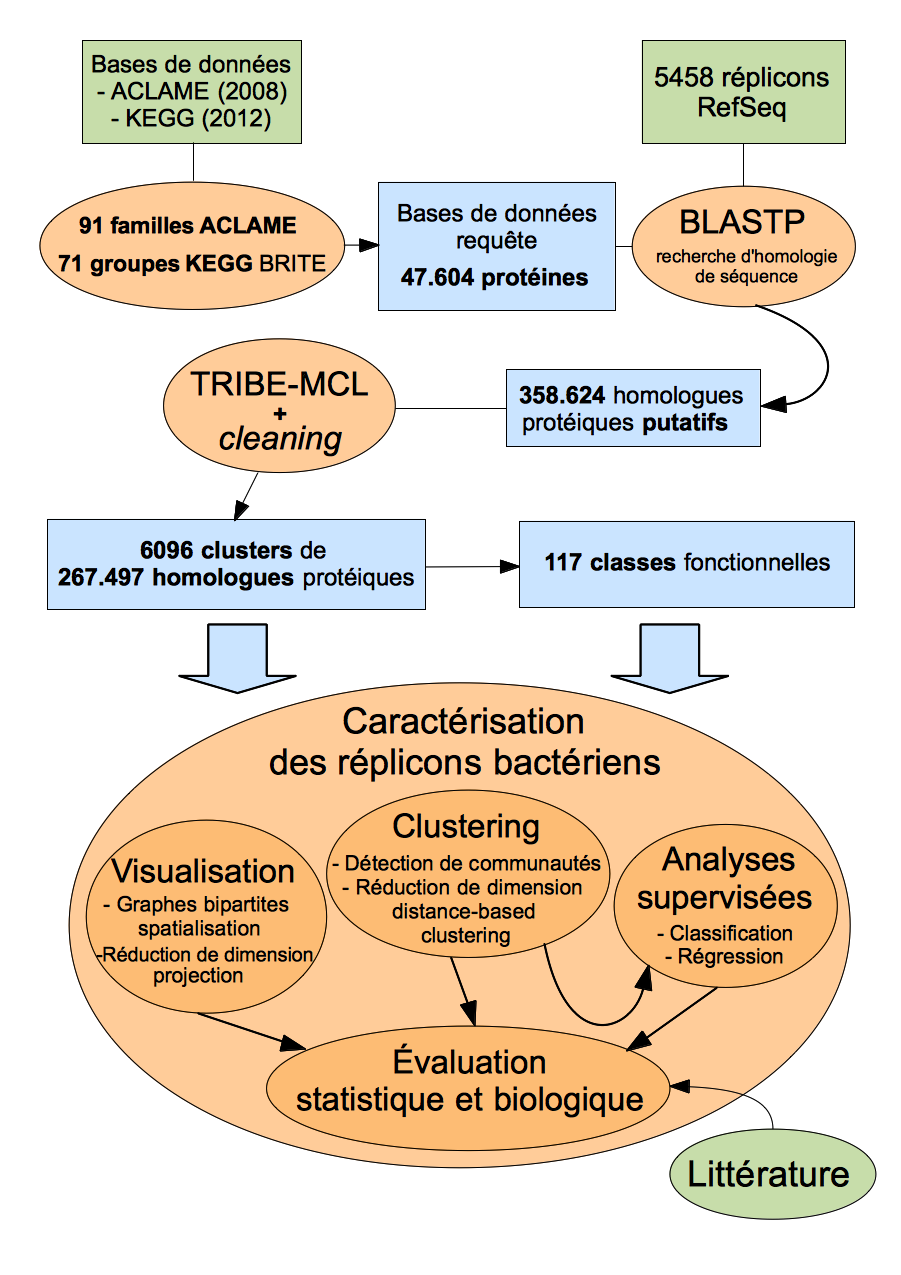
\includegraphics[width=\textwidth]{./img/workflow3.png}
\caption[Pipeline analytique]{Pipeline analytique.}
\end{center}
\end{figure}
